\documentclass[final,twocolumn,5p]{elsarticle}
% \documentclass{sig-alternative}
% \documentclass[conference]{IEEEtran}
% \documentclass[smallextended]{svjour3}
% \documentclass[preprint,12pt,3p,number]{elsarticle}
\usepackage{multirow}
% \usepackage{natbib}
\usepackage{color}
\usepackage{graphics} 
% \usepackage{cite}
\usepackage{rotating}
\usepackage{eqparbox}
\usepackage{graphics}
\usepackage{colortbl} 
%\usepackage{times}
 \usepackage{mathptmx} \usepackage[scaled=.90]{helvet} \usepackage{courier}
\usepackage{balance}
\usepackage{picture}
\usepackage{algorithm}
\usepackage{algorithmicx}
\usepackage{algpseudocode}
\usepackage[export]{adjustbox}
\renewcommand{\footnotesize}{\scriptsize}
\definecolor{lightgray}{gray}{0.8}
\definecolor{darkgray}{gray}{0.6}
\renewcommand{\algorithmicrequire}{\textbf{Input:}}
\renewcommand{\algorithmicensure}{\textbf{Output:}}
%%% graph
\newcommand{\crule}[3][darkgray]{\textcolor{#1}{\rule{#2}{#3}}}
%\newcommand{\rone}{\crule{1mm}{1.95mm}}
%\newcommand{\rtwo}{\crule{1mm}{1.95mm}\hspace{0.3pt}\crule{1mm}{1.95mm}}
%\newcommand{\rthree}{\crule{1mm}{1.95mm}\hspace{0.3pt}\crule{1mm}{1.95mm}\hspace{0.3pt}\crule{1mm}{1.95mm}}
%\newcommand{\rfour}{\crule{1mm}{1.95mm}\hspace{0.3pt}\crule{1mm}{1.95mm}\hspace{0.3pt}\crule{1mm}{1.95mm}\hspace{0.3pt}\crule{1mm}{1.95mm}} 
%\newcommand{\rfive}{\crule{1mm}{1.95mm}\hspace{0.3pt}\crule{1mm}{1.95mm}\hspace{0.3pt}\crule{1mm}{1.95mm}\hspace{0.3pt}\crule{1mm}{1.95mm}}
\newcommand{\quart}[3]{\begin{picture}(100,6)%1
{\color{black}\put(#3,3){\circle*{4}}\put(#1,3){\line(1,0){#2}}}\end{picture}}
\definecolor{Gray}{gray}{0.95}
\definecolor{LightGray}{gray}{0.975}
% \newcommand{\rone}{}
% \newcommand{\rtwo}{}
% \newcommand{\rthree}{}
% \newcommand{\rfour}{} 
% \newcommand{\rfive}{}
\newcommand{\wei}[1]{\textcolor{red}{Wei: #1}} 
\newcommand{\Menzies}[1]{\textcolor{red}{Dr.Menzies: #1}} 

%% timm tricks
\newcommand{\bi}{\begin{itemize}[leftmargin=0.4cm]}
\newcommand{\ei}{\end{itemize}}
\newcommand{\be}{\begin{enumerate}}
\newcommand{\ee}{\end{enumerate}}
\newcommand{\tion}[1]{\S\ref{sect:#1}}
\newcommand{\fig}[1]{Figure~\ref{fig:#1}}
\newcommand{\tab}[1]{Table~\ref{tab:#1}}
\newcommand{\eq}[1]{Equation~\ref{eq:#1}}

%% space saving measures

\usepackage[shortlabels]{enumitem}  
\usepackage{url}
% \def\baselinestretch{1}


% \setlist{nosep}
%  \usepackage[font={small}]{caption, subfig}
% \setlength{\abovecaptionskip}{1ex}
%  \setlength{\belowcaptionskip}{1ex}

%  \setlength{\floatsep}{1ex}
%  \setlength{\textfloatsep}{1ex}
%  \newcommand{\subparagraph}{}

% \usepackage[compact,small]{titlesec}
% \DeclareMathSizes{7}{7}{7}{7} 
% \setlength{\columnsep}{7mm}


\usepackage{graphicx}
\usepackage{multirow}
\usepackage[svgnames]{xcolor}
\usepackage[framed]{ntheorem}
\usepackage{framed}
\usepackage{tikz}
\usetikzlibrary{shadows}
%\newtheorem{Lesson}{Lesson}
\theoremclass{Lesson}
\theoremstyle{break}

% inner sep=10pt,
\tikzstyle{thmbox} = [rectangle, rounded corners, draw=black,
  fill=Gray!20,  drop shadow={fill=black, opacity=1}]
\newcommand\thmbox[1]{%
  \noindent\begin{tikzpicture}%
  \node [thmbox] (box){%
\begin{minipage}{.94\textwidth}%    
      \vspace{-3mm}#1\vspace{-3mm}%
    \end{minipage}%
  };%
  \end{tikzpicture}}

\let\theoremframecommand\thmbox
\newshadedtheorem{lesson}{Result}
\begin{document}
\begin{frontmatter}
\title{ Impacts of Bad ESP (Early Size Predictions) on Software Effort Estimation}
\author{George Mathew\corref{cor1}}
\ead{george.meg91@gmail.com}
\author{Tim Menzies}
\ead{tim.menzies@gmail.com}
\author{Jairus Hihn}
\ead{ jairus.m.hihn@jpl.nasa.gov}
\cortext[cor1]{Corresponding author: Tel:XXX(Wei)}
\address{Department of Computer Science, North Carolina State University, Raleigh, NC, USA,\\
Jet Propulsion Laboratory, Pasadena, CA}



% % \numberofauthors{1}
% \author{Wei Fu \and Tim Menzies \and Xipeng Shen}
% \institute{North Carolina State University, Raleigh, NC, USA
%       Wei Fu \email{w}}
% % \email{fuwei.ee \and tim.menzies@gmail.com \and xshen5@ncsu.edu }

% \thispagestyle{plain}
% \pagestyle{plain}
\begin{abstract}
  \textbf{Context:}
  %For  large systems (e.g.  projects run by government or
%defence departments), it is common to lobby for the development funds prior to commencing the work.
%For such software systems, it is important to have an (approximately) accurate    early lifecycle effort estimate % since (1)~large sums of money are involved and (2)~once funds are allocated, it can be problematic
%to lobby for further funds. However, before the software is built, the size of the final system is not
  %known.
  Boehm cautions that early lifecycle estimates of software size
  can wrong by up to a factor of 400\%. This is a
  major concern for software effort estimation methods that use such ESP
  (\underline{e}arly lifecycle \underline{s}ize \underline{p}redictions)
  for their predictions.\\
  \textbf{Objective:} To understand the impact of  bad ESP on software effort
  estimation. .\\
\textbf{Method:} Explore repositories to determine the space of actual software
size estimation errors seen in practice.  Using the results of the first point, conduct
analytical and perturbation-based  analysis of software
effort models that reply on ESP. \\
\textbf{Results:} (a)~ESP errors are far smaller than   feared by Boehm:
while some
projects have estimate errors over 300\%, most
projects have estiamte errors under  80\%. 
(b)~When perturbing size values within those ranges,
effort models 
only a modest increase in effort estimates error: e.g. 39\% to 44\% in the  median magnitude of relative error. (c)~An analytical evaluation of one effort
model (COCOMO) explains why this might be so:   errors in ESP
are dwarfed by the product of all the other factors.\\
\textbf{Conclusion:} (a)~Bad ESP can lead to poor project effort estimates. (b)~However,
the size of that effect is much less than commonly believed.
(c)~Contrary to prior belief, bad ESP {\em not} the dominate factor leading to inaccurate effort estimates.
\end{abstract}
\end{frontmatter}

% % A category with the (minimum) three required fields
% \vspace{1mm}
% \noindent
% {\bf Categories/Subject Descriptors:} 
% D.2.8 [Software Engineering]: Product metrics;
% I.2.6 [Artificial Intelligence]: Induction

 
\vspace{1mm}
\noindent
{\bf Keywords:} effort estimation, size estimation, parametric models, COCOMO.
%  \maketitle 
\pagenumbering{arabic} %XXX delete before submission

\section{Introduction}
Poor software effort estimation can crippled a project.
In
the worst case, over-running projects are canceled and
the entire development effort is wasted. For example,
NASA canceled its incomplete Check-out Launch Control
System project after the initial \$200M estimate was
exceeded by another \$200M~\cite{clcs03}.

Even after decades of research and model
development, there extensive debates as to which
methods are best.  For example, Shepperd et
al. prefer analogy-based estimation (ABE)
methods~\cite{Shepperd1997}.  Meanwhile, within the
United States Department of Defence and NASA,
parametric effort models like
COCOMO~\cite{Boehm1981} are used extensively and
have found to be quite effective~\cite{Lum2002}.
Also, advocates of agile and devops methods prefer
the planning poker method (discussed in \tion{xxx}).
Finally Jorgensen et al.~\cite{jorgensen09} prefer
expert-based approaches where estimates are derived
by committees of human experts.  For studies
comparing these methods, or how to usefully combine
them, and how to reduce errors when they are used,
see~\cite{koc11b,Minku2013,garg15,me13a,koc11b}.

When these methods are debated, it is usual to discuss problems with {\bf Early Sizing Prediction} (ESP),
specifically:
\begin{quote}
 {\em Is it possible, early in the software lifecycle,
    to accurately estimates the size of the final system?}
  \end{quote}
Note that when such estimates are wrong, then any prediction made from that estimate
will also be wrong. This problem is particularly acute for parametric effort estimation
methods such as Boehm et al.'s COCOMO software effort estimation model.
The core of COCOMO  is an estimate that is exponential on KSLOC (thousands of SLOC); i.e.
\begin{equation}\label{eq:one}
\mathit{effort} \propto \mathit{KSLOC}^{\; n}
\end{equation}
In 1981, Boehm~\cite{boehm81} warned that ESP can be wrong by up to 400\%.
Note that, if such erroneous values were used in \eq{one}, then due to the $ \mathit{KSLOC}^{\; n}$
term, this would lead to  exponentially large errors in the estimate.

Since 1981, much has been learned about software
engineering. Accordingly, it is time to revisit
Boehm's pessimism about bad ESP.  We find that bad SE is far less problematic that suggested
by Boehm.
To show this, this paper explores three research questions
using a simulation study, an analytical study, and a theoretical study.
\bi
\item
{\bf RQ1 (the simulation study): What is the observed impact of bad ESP? }
Given a model producing an estimate, we record the size of the error
in the estimates
after perturbing the size estimates by some factor $\Delta$.
\ei
\begin{lesson}
We find that for the range of $\Delta$ seen in contemporary projects, this error
is usually negligible. That is, 
the
problem of bad ESP is much less than previously
feared.
\end{lesson}
Note that the key part of the {\bf RQ1} analysis is determining the
range of $\Delta$ seen in contemporary projects.
To obtain that range, we used data from 64 recent projects (14 from NASA, 50 
from the United Science Department of Defense). 
This introduces an external validity problem since our answers to {\bf RQ1} are
only good for the values seen in these 64 projects. Therefore, to extend the external
validity of our conclusions:
\bi
\item
{\bf RQ2 (the analytical study):   What is the range of possible effect of bad ESP ?}
For this question, we studied the coeffecients within a parametric effort
estimation model (COCOMO~\cite{boehm81,boehm00b})  to derive minimum and maximum
effects of changes to the KSLOC coeffecient in \eq{one}.
\ei
\begin{lesson}
Given tuning data  from 254 projects, we show that the
  exponential term $n$ is very small: specifically,
  \mbox{$1.06 \le n \le 1.3$}. That is, ESP errors have such a low coefficient that ESP errors
  results in linear, rather than exponential, errors in the predictions.
  \end{lesson}
 The results for {\bf RQ2} is based on more projects than {\bf RQ1}, but it is still
 a small sample from the space of all possible software projects. Accordingly, we conducted
 one more study:
  \bi
  \item
  {\bf RQ3 (the theoretical study): Ignoring all tunings, what is the net
    effect of errors with KSLOC estimation versus errors in other attributes?}
 This theoretical study applies some algebraic manipulations to the COCOMO model
 to derive an expression that comments on the relative effects of KSLOC errors
 to all the other 22 attributes in the COCOMO model.
 \ei
 \begin{lesson}
  Within the COCOMO model,
  KSLOC errors are {\em not} the most influential attribute on effort estimates
 since errors in KSLOC are easily
 dwarfed  by the effects from the other 22 COCOMO attributes.
 \end{lesson}
 Our conclusion from the above is that,
 for the COCOMO model, the results from {\bf RQ1,RQ1,RQ3}  show that there is little reason
  to fear alarmingly large estimation errors due to ESP errors. This is an important contribution since
  one of the standard critiques of COCOMO is its dependency on ESP.

  
  
  The rest of this paper is structured as follows.
  
  \section{Background}
  

 \begin{figure*}[!t]
{\scriptsize
\begin{center}
\begin{tabular}{|p{0.2in}|p{1.46in}|p{1.5in}|p{1.5in}|p{1.5in}|}\hline

 & Definition & Low-end = \{1,2\}
 &Medium =\{3,4\} &High-end= \{5,6\} \\\hline

\multicolumn{1}{c}{~}\\

\multicolumn{5}{l}{Scale factors:}\\\hline
Flex   &  development flexibility   & development process
rigorously defined & some guidelines, which can be relaxed & only
general goals defined\\\hline

Pmat    & process maturity  &  CMM level 1 &   CMM level 3  &  CMM level 5 \\\hline

Prec & precedentedness  &  we have never built this kind
of software before &    somewhat new &
thoroughly familiar \\\hline

Resl &  architecture or risk resolution  &  few interfaces
defined or few risks eliminated  &  most interfaces defined or most
risks eliminated   & all interfaces defined or all risks
eliminated\\\hline

Team  &   team cohesion  &  very difficult interactions &
basically co-operative  &  seamless interactions\\\hline

\multicolumn{1}{c}{~}\\

\multicolumn{5}{l}{Effort multipliers}\\\hline
acap  &  analyst capability  &  worst 35\% &   35\% - 90\% &  best 10\% \\\hline

aexp   &  applications experience  &  2 months &   1 year  &  6 years\\\hline

cplx   &  product complexity   & e.g. simple read/write
statements & e.g. use of simple interface widgets  &  e.g.
performance-critical embedded systems\\\hline

data   &  database size 
(DB bytes/SLOC) &
10 & 100 &    1000 \\\hline

docu   &  documentation   & many life-cycle phases not
documented      & &  extensive reporting for each life-cycle phase\\\hline

ltex   &  language and tool-set experience   & 2 months  &  1
year & 6 years \\\hline

pcap   &  programmer capability  &  worst 15\%   & 55\%  &  best 10\% \\\hline


pcon   &  personnel continuity \newline
(\% turnover per year) &
    48\% &    12\%  & 3\% \\\hline

plex   &  platform experience  &  2 months  &  1 year  &  6 years\\\hline


pvol   &  platform volatility ($\frac{frequency~of~major~changes}{frequency~of~minor~changes}$) &
$\frac{12~months}{1~month}$   & $\frac{6~months}{2~weeks}$ &
$\frac{2~weeks}{2~days}$\\\hline



rely   &  required
reliability &   errors are slight inconvenience  &  errors are easily
recoverable   & errors can risk human life\\\hline




ruse   &  required
reuse &   none &    multiple program  & multiple product lines\\\hline

sced  &   dictated development\newline schedule &    deadlines moved to
75\% of the original estimate &  no change
&  deadlines moved back to  160\% of original estimate\\\hline

site   &  multi-site development   & some contact: phone, mail&
some email  &  interactive multi-media\\\hline

stor  &   required \% of available
RAM & N/A
 &   50\% &  95\% \\\hline


time  &   required \% of available CPU &
N/A&     50\%
   &  95\% \\\hline


tool   &  use of software tools  &  edit,code,debug &&
integrated with life cycle\\\hline

\multicolumn{1}{c}{~}\\

\multicolumn{5}{l}{Effort}\\\hline

months & construction effort  in months& \multicolumn{3}{l|}{1 month =  152 hours (includes development \& management
hours).  
}\\\hline
\end{tabular}
\end{center}
} \caption{COCOMO-II attributes.}
\label{fig:cparems}
\end{figure*}


\subsection{Selection of Model}

For the purposes of this work, we need to explore the effects of ESP errors on some model
of effort estimation. For that work we choose to use the COCOMO model~\cite{boehm81,boehm00b}.
There are two reasons for that selection. Firstly, as shown in \eq{one}, COCOMO seems particularly
susceptible to bad ESP. Secondly, it is widely used in industry and government circles
In our work with the Chinese and the United States software industry,
we saw an   almost exclusive
use  of parametric estimation tools such as those offered by 
Price Systems (pricesystems.com) and  Galorath (galorath.com).
Also,
professional societies, handbooks and
certification programs are mostly developed around 
parametric estimation methods and tools; e.g. see the 
International Cost Estimation and Analysis Society; the
NASA Cost Symposium;  the
International Forum on COCOMO and Systems/Software
Cost Modeling\footnote{See the websites \url{http://tiny.cc/iceaa}, \url{http://tiny.cc/nasa_cost}, \url{http://tiny.cc/csse}}.

  \subsection{COCOMO Details}

  COCOMO was developed in two states: an initial release in 1981~\cite{boehm81}
  followed by an extensive revision in  2000~\cite{boehm00b}.
  In between those releases,
  Boehm created a consortium for
industrial users of COCOMO.
This consortium
collected information on 161 projects from commercial,
aerospace, government, and non-profit organizations.
Using that new data, in 2000, Boehm and his colleagues developed
a set of   {\em tunings} for COCOMO-II that
mapped the project descriptors (very low, low, etc)
into the specific attributes used in the COCOMO model (see \fig{cparems}).
Those tunings, mappings, and attributes became the COCOMO-II model
released 
\begin{equation}\label{eq:cocII}
\mathit{effort}=a\prod_i EM_i *\mathit{KLOC}^{b+0.01\sum_j SF_j}
\end{equation}
Here, {\em EM,SF} are  effort multipliers and scale
factors and
 $a,b$ are the {\em local calibration} parameters (with default values of 2.94 and 0.91).
 In COCOMO-II, effort multipliers change effort by a linear amount
 while scale factors change effort by an exponential amount.
COCOMO-II reports {\em effort}
as ``development months'' where one month
is 152 hours of work  (and includes development and management hours).
For example, if {\em effort}=100, then according to COCOMO,
five developers would finish
the project in 20 months.




 \subsection{Alternatives to COCOMO}

 
COCOMO was initially designed in the age of
waterfall development where projects developed from
requirements to delivery with very little
operational feedback.  Hence, a frequently asked
question about this work is the relevancy of that
$20_{th}$ century software management tool to
current practices.  At issue here is the core
question addressed by this paper.  While there is
nothing inherently ``waterfall'' within the COCOMO
equations, COCOMO does assume that a size estimate
is available before the work starts.  Hence, it is
important to understand when changes to the size of
the software results in inaccurate COCOMO estimates.

Another complaint against the COCOMO equations is
that such ``model-based'' methods are less
acceptable to humans than ``expert-based methods''
were estimated are generated via committees of
experts. The advantage of such expert-based methods
is that if some new project has some important
feature that is not included in the COCOMO
equations, then human expertise can be used to
incorporate that feature into the estimate.
However,
such expert-based approaches have their limitations.
Valerdi~\cite{valerdi11} lists the cognitive biases
that can make an expert offer poor expert-based estimates.
Passos et al. offer specific examples for those
biases: they show that many commercial software
engineers generalize from their first few projects
for all future projects~\cite{passos11}.  J{\o}rgensen
\& Gruschke~\cite{jorgensen09} offer other results
consistent with Passos et al.  when they document
how commercial ``gurus'' rarely use lessons from
past projects to improve their future
expert-estimates.  More generally,
J{\o}rgensen~\cite{Jorgensen2004} reviews studies
comparing model- and expert- based estimation and
concludes that there there is no clear case that
expert-methods are better.  Finally, in 2015,
J{\o}rgensen further argued~\cite{jorg15} that
model-based methods are useful for learning the {\em
  uncertainty} about particular estimates; e.g.  by
running those models many times, each time applying
small mutations to the input data.

 One expert-based estimation method preferred by advocates of
 agile/devops is ``planning poker''~\cite{molokk08}
 where participants offer anonymous ``bids'' on the
 completion time for a project. If the bids are
 widely divergent, then the factors leading to that
 disagreement are elaborated and debated. This cycle
 of bid+discuss continues until a consensus has been
 reached.  Despite having numerous advocates,
 there are very few comparative studies of planning
 poker vs parametric methods. The only direct
 comparison we can find is the 2015 Garg and Gupta
 study that reports planning poker's estimates can be
 twice as bad as those generated via parametric
 methods~\cite{garg15}. One reason for the lack of
 comparisons is that COCOMO and planning poker
 usually address different problems: \bi
\item COCOMO is often used to negotiating resources prior to starting a project;
\item Planning power is often used to adjust current activity within the resource allocation of a project.
  \ei
  Combining these  points, we note that there no real dispute between planning poker (that is an intra-project
task adjustment tool) and COCOMO (which is an pre-project tool for checking if enough resources are available
to start a project).
That said, COCOMO does rely on an early lifecycle size esimate which, according to Boehm~\cite{boehm81}, can be wrong
by up to 400\%.
  \subsection{Problems with Size Estimates}\label{sect:probs}

Size estimates can be expressed in several
forms including function points~\cite{Albrecht83} or  source lines of code (SLOC)~\cite{boehm81}.
No matter how  these size measures are expressed, early in the software development process,
ESP can be inaccurate. For example, here is a list of issues that needs to be resolved before making that
size estimate:
\be
\item How was reused code accounted for in the size estimate?
\item  Was size measured from end-statement or end-of-line?
\item How were lines of comments handled?
\item Given systems built in multiple languages, how were sizes from different programs translated
  into a single number?
\item
  Given some kind of iterative development, how to guess early in the lifecycle
  how much subsequent  feedback will change
  the goals of the project and the size of the delivered system?
  \ee
  The rest of this paper argues that while these five points are {\em potential} problems, in actual fact,
  the net result of these issues is relatively  small (compared to the other sources of error associated with
  COCOMO estimation-- see below for more details).

\section{Three Studies about Bad ESP}
This documents the simulation, analytical, and theoretical studies that address the three
research questions listed in the introduction.
\subsection{RQ1: What is the Observed Impact of Bad ESP?}\label{sect:rq1}
This research question is explored via  a simulation study that
perturbates  size estimates within COCOMO by some random amount $\Delta$.

In order to find valid sizes for $\Delta$, we look to the historical record. 
Two sources were used to learn the typical ranges. Source~\#1 covers fifty projects documented
by Jones \& Hardin~\cite{jones07a} from the United
States Department of Defense.
  While the majority of
these were military-specific applications (command
and control functions), 17 of these are applications
types that could be seen in non-military domains
(see \fig{jones}).
  Further, only a minority of
these ($\frac{15}{50}=30\%$) were waterfall
projects where requirements were mostly frozen prior
to coding: for the remaining 35 of the Jones \& Hardin projects, there was ample opportunity
for scope creep that could lead to inaccuracies in early lifecycle estimates.
\fig{ae} shows the relationship between early lifecycle estimates of SLOC vs final size for the 50
projects of Source~\#1. The diagonal line on that plot shows where the estimate equals the actual.
The key observation from this Source~\#1 data is:
\bi
\item The estimates and actuals are very similar and much less than the 400\% error feared by Boehm in 1981.
  \ei 




\begin{figure}
  \scriptsize
  \begin{center}
      \begin{tabular}{|p{0.77in}|r|r|r|p{0.77in}|}\hline
      Complexity & N &  Product Line  & Environment & State of the Art\\\hline
Simple& 2& Existing& Existing &Current\\
Routine& 10& New& Existing& Current\\
Moderate& 14& New& New& Current\\
Difficult& 24& New& New& New\\\hline
   \end{tabular}

      \vspace{4mm}
      
  \begin{tabular}{|rl|rl|}\hline
        &Application types & &Development processes\\\hline
     31 &Command and Control & 15 &Waterfall\\
    6 &Office Automation, Software Tools, Signals & 12 &Incremental\\
    5 &DFs, Diagnostic, Mission Plans, Sims, Utils; &  8 &Spiral;\\
   5 &Testing; & 15 &Undefined\\
   3 &\multicolumn{3}{l|}{Operating System} \\\hline
  \end{tabular}
  \end{center}
  \caption{50 projects from~\cite{jones07a}.}\label{fig:jones}
  \end{figure}  
Source~\#2 covers 14 projects  from NASA. These projects cover the software used in the deep space
missions of the Jet Propulsion Laboratory. Due to the highly innovative nature of this kind of
software, this final size of this software could easily be incorrected estimated early in its lifecycle.
Many of the details of those NASA systems is proprietary information so, in this article, we cannot describe
the NASA systems at the same level of detail as the Jones \& Hardin sample. What we can show are the ratios
of final/initial SLOC values seen in that code (see \fig{nasaloc}).
 Note
        that none of the values shown here come close to Boehm's ``incorrect by 400\%'' figure;
        in fact- of the 28 estimates shown here, $\frac{24}{28}\approx 86$\%
        only four are more than 80\% incorrect.

 
\begin{figure}
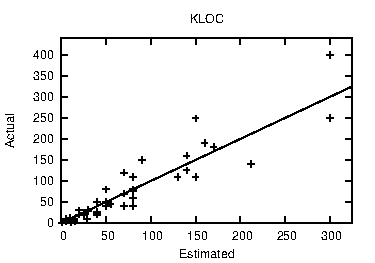
\includegraphics[width=3in]{data.pdf}
\caption{Estimated and actual source lines of code from 50 projects~\cite{jones07a}.}\label{fig:ea}
\end{figure}

 \begin{figure}
      \scriptsize
      \begin{minipage}{.5\linewidth}
      \begin{tabular}{r|rr|}
   project & pre-analysis&pre-coding\\\hline
a&-44\%&-44\%\\
b&-13\%&-4\%\\
c&-6\%&-6\%\\
d&-4\%&-4\%\\
e&5\%&5\%\\
e&7\%&\\
f&10\%&10\%\\
g&54\%&54\%\\
h&64\%&64\%\\
i&69\%&69\%\\
j&78\%&78\%\\
k&95\%&52\%\\
l&206\%&10\%\\
m&236\%&236\%
      \end{tabular}\end{minipage} \begin{minipage}{.33\linewidth}
        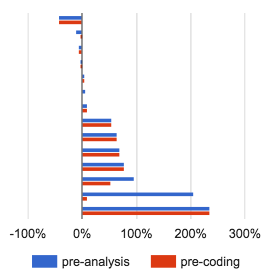
\includegraphics[width=1.8in]{nasadata.png}
        \end{minipage}
      \caption{Errors in estimates of final system size (measured in terms of LOC)
        seen before analysis and coding in 14 NASA projects. Values in the left-hand-size table
        are shown graphically at right.
        All percentages here are percents on the final code size. For example, in the last
        line, Project M's final size was 236\% larger than predicted at the pre-analysis stage.
        Positive values denote initial under-estimates while negative values denote over-estimates
        (e.g. the size of the first four projects were initially over-estimated).}
        \label{fig:nasaloc}
    \end{figure}


 
\begin{figure}
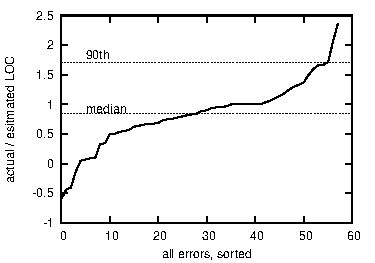
\includegraphics[width=3in]{all.pdf}
\caption{All errors seen in our two sources. 50th and 90th percentile on those errors are 91\% and 170\%.}\label{fig:allerr}
\end{figure}

\fig{allerr} sorts all the {\em final/initial} ratios from our two sources. The horizontal lines in those figures show
the 50th and 90th value in that sort:
\bi
\item The median 50th percentile error is 91\%;
 \item The outlier 90th percentile error is 170\%.
   \ei
   Based on \fig{allerr}, we say that if perturb SLOC estimates by plus or minus 200\% then that more than covers the typical
   values seen in the historical record.

   \subsection{RQ2: Is there a tolerance limit for ESP?}\label{sect:rq2}

\begin{figure}[!t]
\begin{lstlisting}
_  = None;  Coc2tunings = [[
#              vlow  low   nom   high  vhigh  xhigh   
# scale factors:
'Flex',        5.07, 4.05, 3.04, 2.03, 1.01,     _],[
'Pmat',        7.80, 6.24, 4.68, 3.12, 1.56,     _],[
'Prec',        6.20, 4.96, 3.72, 2.48, 1.24,     _],[
'Resl',        7.07, 5.65, 4.24, 2.83, 1.41,     _],[
'Team',        5.48, 4.38, 3.29, 2.19, 1.01,     _],[
# effort multipliers:        
'acap',        1.42, 1.19, 1.00, 0.85, 0.71,    _],[
'aexp',        1.22, 1.10, 1.00, 0.88, 0.81,    _],[
'cplx',        0.73, 0.87, 1.00, 1.17, 1.34, 1.74],[
'data',           _, 0.90, 1.00, 1.14, 1.28,    _],[
'docu',        0.81, 0.91, 1.00, 1.11, 1.23,    _],[
'ltex',        1.20, 1.09, 1.00, 0.91, 0.84,    _],[
'pcap',        1.34, 1.15, 1.00, 0.88, 0.76,    _],[ 
'pcon',        1.29, 1.12, 1.00, 0.90, 0.81,    _],[
'plex',        1.19, 1.09, 1.00, 0.91, 0.85,    _],[ 
'pvol',           _, 0.87, 1.00, 1.15, 1.30,    _],[
'rely',        0.82, 0.92, 1.00, 1.10, 1.26,    _],[
'ruse',           _, 0.95, 1.00, 1.07, 1.15, 1.24],[
'sced',        1.43, 1.14, 1.00, 1.00, 1.00,    _],[ 
'site',        1.22, 1.09, 1.00, 0.93, 0.86, 0.80],[ 
'stor',           _,    _, 1.00, 1.05, 1.17, 1.46],[
'time',           _,    _, 1.00, 1.11, 1.29, 1.63],[
'tool',        1.17, 1.09, 1.00, 0.90, 0.78,    _]]

def COCOMO2(project,  a = 2.94, b = 0.91, # defaults
                      tunes= Coc2tunings):# defaults 
  sfs ems, kloc  = 0,1,22          
  scaleFactors, effortMultipliers = 5, 17
  for i in range(scaleFactors):
    sfs += tunes[i][project[i]]
  for i in range(effortMultipliers):
    j = i + scaleFactors
    ems *= tunes[j][project[j]] 
  return a * ems * project[kloc] ** (b + 0.01*sfs) 
\end{lstlisting}
\caption{COCOMO-II: effort estimates from a {\em project}.
Here, {\em project} has up to 24 attributes  (5 scale
factors plus 17 effort multipliers plus KLOC plus. in the training data, the actual effort).
Each attribute except KLOC and effort is scored
using the scale very low = 1, low=2, etc.
For an explanation of the attributes shown in
green, see \fig{cparems}.}\label{fig:coc2}
\end{figure}



To conduct the perturbation study for identifying a point of tolerance,  we use  COCOMO since its internal details have been fully published~\cite{boehm00b}. Also, we can access a full implementation of the  2000 COCOMO model. Further, we have access to four interesting  COCOMO data sets. With one exception, our learning experiments do not use the data that generated   standard COCOMO. That exception is the  COC81 data-- which  lets us  compare new methods against the  labor intensive methods used to make standard COCOMO-- see \fig{dataused}.

The primary method used in our study is the COCOMO2 which is described using simple python code in \fig{coc2}. The impact of noise in \textit{KLOC} is studied by varying $\mathit{KLOC}$ as follows

\begin{equation}
    \label{eq:kloc}
    \mathit{KLOC} = \mathit{KLOC}*((1- n) + (2*n*r))
\end{equation}

where $n \in [0.2, 0.4, 0.6, 0.8, 1.0]$ is the level of noise we are exploring and $r$ is a random number
$0 \le r \le 1$. In the results, any result
prefixed with {\em 0.2} to {\em 1.0} shows what happens
when the KLOCs were varied by 20\% to 100\% respectively.

\begin{figure*}[!ht]
    \centering
    \begin{minipage}[c]{\linewidth}
    \begin{mdframed}
    Scott-Knott procedure recommended by Mittas \& Angelis in their 2013 IEEE TSE paper~\cite{mittas13}.  This method sorts a list of $l$ treatments with $ls$ measurements by their median score. It then splits $l$ into sub-lists $m,n$ in order to maximize the expected value of differences  in the observed performances before and after divisions. E.g. for lists $l,m,n$ of size $ls,ms,ns$ where $l=m\cup n$:
     \[E(\Delta)=\frac{ms}{ls}abs(m.\mu - l.\mu)^2 + \frac{ns}{ls}abs(n.\mu - l.\mu)^2\]

    Scott-Knott then applies some statistical hypothesis test $H$ to check if $m,n$ are significantly different. If so, Scott-Knott then recurses on each division.Scott-Knott is better than an all-pairs hypothesis test of all methods; e.g. six treatments can be compared \mbox{$(6^2-6)/2=15$} ways.  A 95\% confidence test run for each comparison has  a very low total confidence: \mbox{$0.95^{15} = 46$}\%. To avoid an all-pairs comparison, Scott-Knott only calls on hypothesis tests {\em after} it has found splits that maximize the performance differences.

    For this study, our hypothesis test $H$ was a conjunction of the A12 effect size test(endorsed by Arcuri \etal in ICSE '11 \cite{arcuri11}) of  and non-parametric bootstrap sampling \cite{efron93}; i.e. our Scott-Knott divided the data if {\em both}
    bootstrapping and an effect size test agreed that the division was statistically significant (99\% confidence) and not a ``small'' effect ($A12 \ge 0.6$). 
    For a justification of the use of non-parametric
    bootstrapping, see Efron \&
    Tibshirani~\cite[p220-223]{efron93}.
    For a justification of the use of effect size tests
    see Shepperd \& MacDonell~\cite{shepperd12a}; Kampenes~\cite{kampenes07}; and
    Kocaguneli et al.~\cite{kocharm13}. These researchers
    warn that even if an
    hypothesis test declares two populations to be
    ``significantly'' different, then that result is
    misleading if the ``effect size'' is very small.
    Hence, to assess 
    the performance differences 
    we first must rule out small effects.
    Vargha and Delaney's
    non-parametric 
    A12 effect size test 
    explores
    two lists $M$ and $N$ of size $m$ and $n$:
    \[A12 = \left(\sum_{x\in M, y \in N} 
    \begin{cases} 
    1   & \mathit{if}\; x > y\\
    0.5 & \mathit{if}\; x == y
    \end{cases}\right) / (mn)
    \]
    This expression computes the probability that numbers in one sample are bigger than in another.
    This test was recently 
    endorsed by Arcuri and Briand
    at ICSE'11~\cite{arcuri11}.
    \end{mdframed}
    \caption{Scott-Knott Test}
    \end{minipage}
    \label{fig:sk}
\end{figure*}

% Please add the following required packages to your document preamble:
% \usepackage{multirow}
\begin{figure}[!t]
\begin{center}
\caption{NASA10}
\scriptsize
\label{fig:nasa10}
\begin{tabular}{|r|c|c|c|c|}
\hline
\multicolumn{1}{|c|}{\multirow{2}{*}{\textbf{Name}}} & \multicolumn{2}{c|}{\textbf{Med}}     & \multicolumn{2}{c|}{\textbf{IQR}} \\ \cline{2-5} 
\multicolumn{1}{|c|}{}                               & \textbf{Rank} & \textbf{Med $\pm$ IQR} & \textbf{Rank} & \textbf{Med $\pm$ IQR} \\ \hline
    COCOMO2  & 1 & 43 $\pm$ 48   & 1    & 1 $\pm$ 1     \\ \cline{4-5}
20\%:COCOMO2 & 1 & 41 $\pm$ 57   & 2    & 13 $\pm$ 19   \\ \cline{4-5}
40\%:COCOMO2 & 1 & 41 $\pm$ 50   & 3    & 28 $\pm$ 14   \\ \cline{2-3}
60\%:COCOMO2 & 2 & 46 $\pm$ 54   & 3    & 34 $\pm$ 44   \\ 
80\%:COCOMO2 & 2 & 50 $\pm$ 54   & 3    & 44 $\pm$ 39   \\
100\%:COCOMO2 & 2 & 68 $\pm$ 59  & 3    & 49 $\pm$ 32    \\ \hline         
\end{tabular}


\caption{COC05}
\scriptsize
\label{fig:coc05}
\begin{tabular}{|r|c|c|c|c|}
\hline
\multicolumn{1}{|c|}{\multirow{2}{*}{\textbf{Name}}} & \multicolumn{2}{c|}{\textbf{Med}}     & \multicolumn{2}{c|}{\textbf{IQR}} \\ \cline{2-5} 
\multicolumn{1}{|c|}{}                               & \textbf{Rank} & \textbf{Med $\pm$ IQR} & \textbf{Rank} & \textbf{Med $\pm$ IQR} \\ \hline
    COCOMO2  & 1 & 13 $\pm$ 53   & 1    & 1 $\pm$ 1     \\ \cline{4-5}
20\%:COCOMO2 & 1 & 14 $\pm$ 53   & 2    & 8 $\pm$ 22   \\ 
40\%:COCOMO2 & 1 & 19 $\pm$ 50   & 2    & 14 $\pm$ 42   \\ \cline{2-5}
60\%:COCOMO2 & 2 & 24 $\pm$ 57   & 3    & 25 $\pm$ 67   \\ 
80\%:COCOMO2 & 2 & 25 $\pm$ 46   & 3    & 25 $\pm$ 79   \\
100\%:COCOMO2 & 2 & 26 $\pm$ 71  & 3    & 30 $\pm$ 96    \\ \hline    
\end{tabular}

\caption{NASA93}
\scriptsize
\label{fig:nasa93}
\begin{tabular}{|r|c|c|c|c|}
\hline
\multicolumn{1}{|c|}{\multirow{2}{*}{\textbf{Name}}} & \multicolumn{2}{c|}{\textbf{Med}}     & \multicolumn{2}{c|}{\textbf{IQR}} \\ \cline{2-5} 
\multicolumn{1}{|c|}{}                               & \textbf{Rank} & \textbf{Med $\pm$ IQR} & \textbf{Rank} & \textbf{Med $\pm$ IQR} \\ \hline
    COCOMO2  & 1 & 14 $\pm$ 39   & 1    & 1 $\pm$ 2     \\ \cline{4-5}
20\%:COCOMO2 & 1 & 14 $\pm$ 40   & 2    & 5 $\pm$ 8   \\ \cline{4-5}
40\%:COCOMO2 & 1 & 15 $\pm$ 43   & 3    & 8 $\pm$ 14   \\ \cline{4-5}
60\%:COCOMO2 & 1 & 16 $\pm$ 44   & 4    & 12 $\pm$ 24   \\ \cline{2-3}
80\%:COCOMO2 & 2 & 20 $\pm$ 40   & 4    & 13 $\pm$ 28   \\\cline{4-5}
100\%:COCOMO2 & 2 & 27 $\pm$ 42  & 5    & 19 $\pm$ 36    \\ \hline  
\end{tabular}

\caption{COC81}
\scriptsize
\label{fig:coc81}
\begin{tabular}{|r|c|c|c|c|}
\hline
\multicolumn{1}{|c|}{\multirow{2}{*}{\textbf{Name}}} & \multicolumn{2}{c|}{\textbf{Med}}     & \multicolumn{2}{c|}{\textbf{IQR}} \\ \cline{2-5} 
\multicolumn{1}{|c|}{}                               & \textbf{Rank} & \textbf{Med $\pm$ IQR} & \textbf{Rank} & \textbf{Med $\pm$ IQR} \\ \hline
    COCOMO2  & 1 & 3 $\pm$ 18   & 1    & 0 $\pm$ 1     \\ \cline{4-5}
20\%:COCOMO2 & 1 & 4 $\pm$ 20   & 2    & 2 $\pm$ 4   \\ \cline{4-5}
40\%:COCOMO2 & 1 & 4 $\pm$ 16   & 3    & 4 $\pm$ 7   \\ \cline{2-5}
60\%:COCOMO2 & 2 & 6 $\pm$ 19   & 4    & 6 $\pm$ 11   \\ \cline{4-5}
80\%:COCOMO2 & 2 & 6 $\pm$ 21   & 5    & 7 $\pm$ 15   \\
100\%:COCOMO2 & 2 & 8 $\pm$ 18  & 5    & 8 $\pm$ 18    \\ \hline        
\end{tabular}
\end{center}
\end{figure}

\begin{figure}
    \centering
    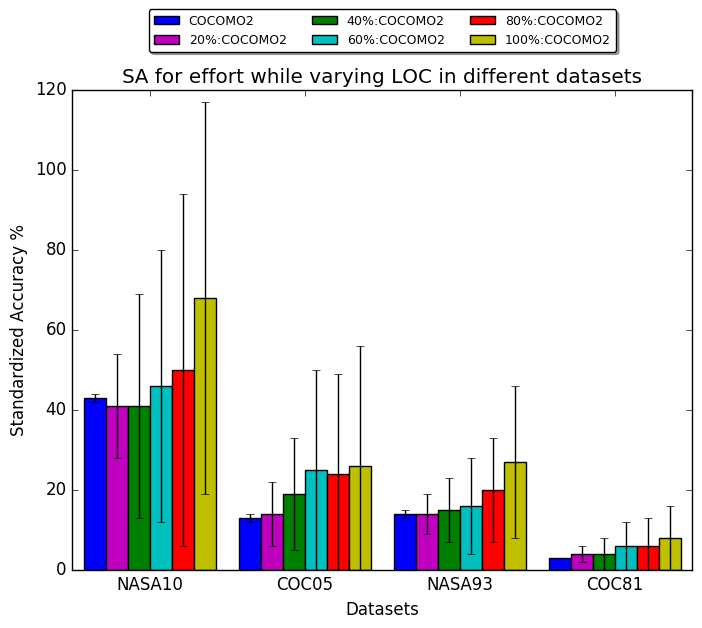
\includegraphics[scale=0.45]{Figs/sa.png}
    \caption{Standarized Accuracy for effort while varying LOC in different datasets.}
    \label{fig:sa_datasets}
\end{figure}

% \begin{equation}\label{eq:mre}
% \mbox{$ \mathit{MRE}=\frac{abs(\mathit{actual} - \mathit{predicted})}{\mathit{actual}}$}
% \end{equation}

\begin{equation}\label{eq:sa}
\mbox{$ \mathit{SA}=\frac{abs(\mathit{actual} - \mathit{predicted})}{\mathit{\sum_{i=1}^{1000}|\pmb{choice}(all) - predicted|}/1000}$}
\end{equation}

Each of the four tables(\fig{nasa10}, \fig{coc05}, \fig{nasa93} \& \fig{coc81}) represent Standardized Accuracy(SA) values seen in leave-one-out-studies, repeated twenty times for the dataset highlighted in table\'s title. i.e. For every project in a dataset, the value of $r$ from \eq{kloc} is changed 20 times and KLOC is estimated and then substituted in \eq{one}. SA is calculated as shown in \eq{sa} where $actual$ is the true value of effort, $predicted$ is the estimated value, $all$(array) is all the effort values in the dataset and $\pmb{choice}$ randomly picks one value from an array.  The first column in each table denotes the name of the method. COCOMO2 represents estimating effort using COCOMO-II as shown in \fig{coc2}. $x$\%:COCOMO2 represents COCOMO-II where KLOC is perturbed with an error of $x$\% using \eq{kloc}. Column 3 highlights the median and IQR for the median of the SA while column 5 highlights the median and IQR of the IQR of SA.  {\em Better} methods appear {\em higher} in the tables.In these tables, median and IQR are the 50th and the  (75-25)th percentiles. Horizontal lines divide the ``ranks'' found by our Scott-Knott+bootstrapping+effect size tests (shown in column ``Rank''). In these tables we can observe that upto 40\% error in $KLOC$ is tolerable and error greater than that significantly changes the estimate. This observation is further backed by \fig{sa_datasets} which graphically show how the SA changes as we increase the error for the 4 datasets. Thus, there is point of tolerance beyond which estimation error increases significantly.
    
   \subsection{RQ3: What is the range of possible effects of bad ESP ?}\label{sect:rq3}
 This analytical study  of this section  examines the coefficients of the terms in the COCOMO equation
 to see what effect changes in KSLOC have on COCOMO's effort prediction.
 This study is motivated as follows:
 \bi
 \item
 Recall
from the introduction that this exponential nature of the COCOMO equation 
made it seem as if COCOMO would be most suceptible to errors in lines of code.
\item
Yet we saw in the last section that COCOMO is remarkably {\em insensitive} to LOC errors.
\ei
One explanation for the strange results of the last section is that the coeffecients
on the exponential term in   COCOMO   are so small that COCOMO does not
react poorly to LOC errors.
The analytical study of this section shows that this is indeed the case. In turns
out that for most projects, the COCOMO effort estimate is effectively linear, and not exponential
on SLOC.
The proof of this is somewhat somewhat technical but the main result is \eq{sf3} 
that shows the range  of the exponential coefficients for  COCOMO projects. Note that rarely are those coefficients very very large-- so much so that when we graph the changes in effort due to increased SLOC, the scale-up
is much less than exponential (see \fig{lowerupper}).



The coeffecients learned by Boehm in 2000 for the
COCOMO were based on an analysis of 
161 projects from commercial, aerospace, government, and non-profit organizations~\cite{boehm00b}. At the time of that analysis,
those  projects   were of size 20 to 2000 KSLOC (thousands of lines of code) and took between 100 to 10000 person months to build.
Recall from \eq{one} that that work concluded that, in COCOMO
\begin{equation}\label{eq:zero}
\mathit{effort} \propto \mathit{KSLOC}^{\;x}
\end{equation}
where 
\begin{equation}\label{eq:sum1}
x={b + 0.01 \sum_i SF_i}
\end{equation}
Boehm's   $SF_i$ coeffecients
are presented in a table inside the front cover of the COCOMO-II text~\cite{boehm00a}(see \fig{coc2}).
When
  projects have ``very low'', ``low'', ``nominal'', ``high'', ``very high'' values in the COCOMO , then from that table it can be see that:
\begin{equation}\label{eq:sf1}
\begin{array}{r|l}
  &0.01 \sum_i  SF_i \\\hline
\mathit{very\; low} & 0.32\\
\mathit{  low} &   0.25\\
\mathit{nominal} &  0.192\\
\mathit{high} &  0.13\\
\mathit{very\; high} &  0.06  
\end{array}
\end{equation}
In 2000, Boehm proposed default values for $a,b$= $2.94,0.91$.
Those ranges of   where checked    by Baker~\cite{baker07} 
using 92 projects from NASA's Jet Propulsion Laboratory\footnote{As mentioned
above, these 92 projects do not overlap with Boehm's 161 projects}.  Recall from \eq{cocII}
that the $a,b$ local calibration parameters can be adjusted using local data. 
Baker checked those ranges by,  30 times, running the COCOMO
calibration procedure using 90\% of the JPL data (selected
at random). He reported that
 $a$ was approximately linearly related to $b$ as follows:
\[
\begin{array}{c}
\left(2.2 \le a \le 9.18\right) \bigwedge  \left(b(a,r) = -0.03a + 1.46 + r*0.1\right)
\end{array}
\]
Note that Baker's found ranges for $a$ included the $a=2.94$ value proposed by Bohem.

In the  above,  ``r'' is a random number $0 \le r \le 1$ so Baker's maximum and minimum $b$ values
were:
\[
\begin{array}{c}
b(2.2,\; 0) = 1.394\\
b(9.18,\; 1) =1.2846
\end{array}
\]
Combined with Boehm's default values for $b=0.91$, we say that in the historical record
there is evidence for $b$ ranging
\begin{equation}\label{eq:sf2}
0.91 \le b \le 1.394
\end{equation}
Combining \eq{sum1}, \eq{sf1}, \eq{sf2} we see that the coeffiecent on the 
KSLOC term in \eq{zero} is 
\begin{equation}\label{eq:sf3} 
\begin{array}{r|l}
                  &  x= b + 0.01 \sum_i SF_i \\\hline
\mathit{very\; low} &  1.22 \le x \le 1.71\\
\mathit{  low} &  1.16 \le x \le 1.65 \\
\mathit{nominal}& 1.10 \le x \le 1.58    \\
\mathit{high} &  1.04 \le x \le 1.52  \\
\mathit{very\; high} & 0.97 \le x \le 1.46   
\end{array}
\end{equation} 
\fig{lowerupper} shows   $\mathit{effort} = \mathit{KLOC}^x$ results using the coeffecients
of \eq{sf3}. Note that the vertical axis of that chart a logarithmic scale.
On such a scale, an function that is exponential on the horizontal access will
appear as a straight line. All these plots bent over to the right; i.e. even
under the most pessimist  assumptions (see ``very low'' for ``upper bound''), the
effect of LOC on effort in COCOMO is far less than exponential-- an observation
that explains why in \tion{rq1} COCOMO's estimates were not dramatically altered
by errors in LOC.

\begin{figure}[!t] 
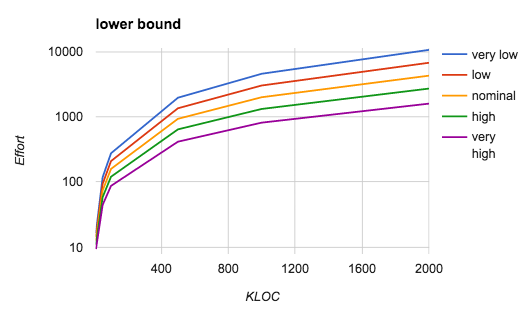
\includegraphics[width=3.5in]{Figs/lower.png}


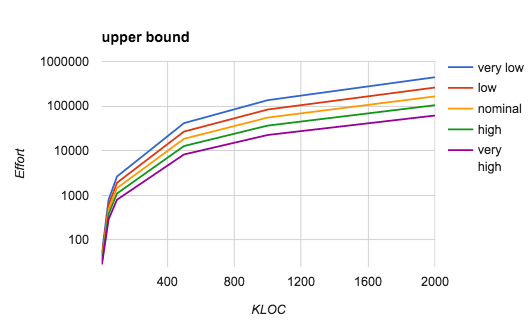
\includegraphics[width=3.5in]{Figs/upper.png} 
\caption{Growth in effort estimates as source code grows. Growth rate determined by \eq{sf3}. 
``Lower bound'' is the most optimistic projection (effort grows slowest as LOC increases)
while ``Upper bound is most pessimistic.
For example, in `upper bound'' for ``very low'', $\mathit{effort} = \mathit{KLOC}^{1.71}$ (where 1.71 is the top-right figure of \eq{sf3}. }\label{fig:lowerupper}
\end{figure}
 


\subsection{RQ4: What is the net effect of errors with KSLOC on estimation
versus error in other attributes?}\label{sect:rq4}


Note that, from \eq{cocII},
the minimum  
effort  is bounded by the  {\em sum} of the minimum scale factors
and the {\em product} of the minimum effort multipliers.
Similar expressions hold for the  maximum effort estimate. Hence,
for a given KLOC, the range of values is given by:
\[
0.057*\mathit{KSLOC}^{0.97}  \le \mathit{effort} \le 115.6*\mathit{KSLOC}^{1.71}\]
(The exponents in the this expression come from \eq{sf3}. The linear terms come
from the product of the min/max effort multipliers from the 
the COCOMO-II text~\cite{boehm00b}).

Dividing the minimum and maximum values results in an  expression showing
how    effort can vary for any given KLOC due to variations in the effort multipliers
and scale factors: 
\begin{equation}\label{eq:ration}
115.6/0.057 *\mathit{KSLOC}^{1.71 - 0.97} = 2028*\mathit{KSLOC}^{0.74}
\end{equation}
Note the very large linear term (2028) coming from the effort multipliers and the
small exponential term (0.74) coming from the scale factors that acts on the KSCOC estimate. The lesson of \eq{ration}
is that errors in KSLOC can have less of an impact on effort predictions than
errors in COCOMO's effort multipliers. Hence, as seen in \tion{rq1}, it is possible
that errors in KSLOC will not be a major cause of estimatione errors.

 
  

\section{Validity}

\subsection{Sampling Bias}
The analysis process described above was designed specifically to
address issues of sampling bias.   The simulation study of \tion{rq1} perturbed SLOC values according to the ranges found
in 64 projects. Hence, the conclusions of \tion{rq1} are heavily biases by that sample.

The other studies shown in \tion{rq2} and \tion{rq3} were based on more data (253 projects) than the simulations study.  That study
found that even if the LOC errors were larger than those documented in \tion{rq1}, then the net effect of 
those errors would not be disastrous since, given domain tunings,   KSLOC  errors are  not especially exponentially associated with effort errors. 
 


\subsection{External Validity}

One clear bias in this study is the use of the COCOMO model for studying the effects
of LOC errors on estimates. Our case for using COCOMO was made above in {\S}2: 
(a)~COCOMO s widely used in industry and government circles in the United States and China;
(b)~COCOMO's assumption that effort is exponentially proportional to SLOC seems to make it
exponentially sensitive to errors in SLOC estimates. 

As to external validity of our conclusions for  other effort estimation methods, we leave that for future work.
  That said, the methods of this paper could used be used to  certify that some effort
  estimator  is not prone to bad ESP
  errors.  The simulation study described above
   could be applied to any other
   effort estimation method. Also, for parametric estimation methods, it would also be possible to apply
   the theoretical study and the analytical study  (caveat: but
   note that the analytical study requires access to project data in order to understand the space of
  usual model values).
  
  

  
  
\section{Conclusion}
Prior work raised alarms about problems with generating early life cycle estimates of software
development effort. Boehm~\cite{boehm81} cautioned that such early estimates can be wrong by a factor of up to  400\%.

While that may have been true in 1981, in 2016 we have found much evidence that we can be far more optimistic about
our ability to generate reasonably accurate early lifecycle estimates:
\bi
\item
ESP errors seen in practice are much smaller than previously feared. Nowhere in
this study did we find errors of order of ``plus or minus 400\%'', as feared
by Boehm in 1981. In fact, look at \fig{allerr}, the median ESP error we found in
this study are around -10\% (i.e. we typicallt over-estiamte the size of our software, by a small amount).
\item
When we perturb LOC values within effort predictors, we find that within the ranges
of \fig{allerr}, the net effect of those perturbations is very small. We documented that result above via simuation studies (in \tion{rq1}) and an analytical study of the SKLOC coeffecients with an effort estimator (in \tion{rq2}).
\item
Effort estimators
use size measures, and many other values, to produce their predictions.  When we
pare the effects of SKLOC error relative to errors in the other project
descriptors (in \tion{rq3}), we find that KLSOC errors can be relatively less 
influential than the errors in the dozens of attributes in a model.
\ei
The last point is particularly significant. While there are many reasons why ESP can fail (see \tion{probs}),
as shown above, the net impact of those errors is relatively small. The results of \tion{rq3}
show that it is important to consider all the attributes used by  effort model, not just LOC.  
Future work should focus on how to better collect more accurate information about (e.g.)
the attributes are shown in \fig{cparem}.  

\section*{Acknowledgments}
The work has partially funded by a National Science Foundation CISE CCF award \#1506586.
 
\vspace*{0.5mm}
 
 
% \bibliographystyle{plain}
\bibliographystyle{elsarticle-num}
% \balance
\bibliography{refs}  

   



%   %%%%parameters for F %%%%%%
% \begin{table*}[!ht]
 
% \resizebox{\textwidth}{!}{
% % \renewcommand{\baselinestretch}{0.9}
% \scriptsize
% \centering
%   \begin{tabular}{|c |c |c |c |c |c |c |c |c |c |c |c |c |c |c |c |c |c |c |c |}
%     \hline
    
%   \begin{tabular}[c]{@{}c@{}}Learner \\ Name\end{tabular}&Parameters  & Default &antV0&antV1&antV2&camelV0&camelV1&ivy&jeditV0&jeditV1&jeditV2&log4j&lucene&poiV0&poiV1&synapse&velocity&xercesV0&xercesV1\\ 
%  \hline
% \multirow{8}{*}{\begin{tabular}[c]{@{}c@{}}Where\\based\\ Learner\end{tabular}}
% & threshold& 0.5& 0.04& 0.44& 0.44& 0.98& 0.65& 0.77& 1& 0.65& 0.98& 0.44& 0.44& 0.87& 0.04& 0.77& 0.24& 0.44& 0.77\\ \cline{2-20}
% & infoPrune& 0.33& 0.51& 0.68& 0.88& 0.47& 0.07& 0.31& 0.48& 0.68& 0.57& 0.12& 0.68& 0.01& 0.51& 0.14& 0.54& 0.68& 0.14\\ \cline{2-20}
% & min\_sample\_size& 4& 6& 4& 6& 1& 6& 8& 8& 4& 6& 7& 4& 9& 6& 2& 8& 4& 8\\ \cline{2-20}
% & min\_Size& 0.5& 0.18& 0.4& 0.56& 0.51& 0.65& 0.59& 0.97& 0.4& 0.51& 0.8& 0.4& 0.77& 0.18& 0.62& 0.46& 0.4& 0.66\\ \cline{2-20}
% & wriggle& 0.2& 0.25& 0.29& 0.76& 0.6& 0.63& 0.26& 1& 0.51& 0.17& 0.36& 0.51& 0.83& 0.25& 0.5& 0.52& 0.29& 0.26\\ \cline{2-20}
% & depthMin& 2& 3& 3& 3& 1& 5& 3& 2& 3& 5& 5& 3& 4& 3& 3& 3& 3& 3\\ \cline{2-20}
% & depthMax& 10& 16& 15& 15& 8& 19& 10& 7& 15& 5& 15& 15& 19& 16& 6& 19& 15& 10\\ \cline{2-20}
% & wherePrune& False& False& True& True& True& True& True& True& False& False& True& True& True& False& True& False& False& True\\ \cline{2-20}
% & treePrune& True& False& True& True& False& False& False& False& False& True& True& True& False& False& False& True& True& False\\ \cline{2-20}
% \hline
% \multirow{5}{*}{CART}
% & threshold& 0.5& 0.34& 0.25& 0.01& 0.01& 0.73& 0.53& 0.92& 0.8& 0.74& 0.54& 0.03& 0.91& 0.01& 0.01& 0.55& 1& 0.01\\ \cline{2-20}
% & max\_feature& None& 0.01& 0.01& 0.29& 0.01& 0.46& 0.75& 0.79& 0.74& 0.41& 0.81& 0.61& 0.72& 0.01& 0.01& 0.01& 0.25& 0.18\\ \cline{2-20}
% & min\_samples\_split& 2& 18& 20& 12& 2& 15& 11& 2& 18& 13& 9& 17& 16& 10& 4& 8& 3& 15\\ \cline{2-20}
% & min\_samples\_leaf& 1& 19& 16& 15& 17& 1& 1& 13& 10& 4& 3& 7& 5& 20& 7& 8& 1& 6\\ \cline{2-20}
% & max\_depth& None& 12& 2& 15& 1& 41& 20& 44& 15& 13& 5& 23& 14& 1& 5& 17& 47& 13\\ \cline{2-20}
% \hline
% \multirow{6}{*}{\begin{tabular}[c]{@{}c@{}}Random \\ Forests\end{tabular}} 
% & threshold& 0.5& 0.01& 0.35& 0.3& 0.01& 0.9& 0.97& 0.63& 1& 0.73& 0.68& 0.01& 1.0& 0.01& 0.07& 0.22& 1& 0.82\\ \cline{2-20}
% & max\_feature& None& 0.63& 0.17& 0.01& 0.01& 0.88& 0.74& 0.76& 0.73& 0.01& 0.03& 0.39& 0.02& 0.01& 0.56& 0.36& 0.51& 0.89\\ \cline{2-20}
% & max\_leaf\_nodes& None& 40& 33& 46& 22& 11& 16& 38& 34& 30& 31& 12& 49& 25& 47& 15& 39& 24\\ \cline{2-20}
% & min\_samples\_split& 2& 10& 16& 20& 1& 1& 1& 1& 4& 20& 19& 11& 14& 2& 17& 19& 20& 19\\ \cline{2-20}
% & min\_samples\_leaf& 1& 4& 15& 9& 13& 18& 11& 3& 16& 17& 6& 10& 7& 19& 13& 11& 2& 14\\ \cline{2-20}
% & n\_estimators& 100& 120& 73& 75& 130& 97& 144& 125& 97& 80& 111& 96& 101& 50& 67& 74& 63& 66\\ \cline{2-20}
% \hline  \end{tabular}
% }
%   \caption{Parameters tuned on different models over the objective of ``F''.}\label{tab:fselect}
% \end{table*}
 
  
% \clearpage
% \pagenumbering{roman}
% \setcounter{page}{1} 
% \section*{Reply to Reviews}

% Thank your for your comments. The typos listed by reviewers
% have been fixed and the remainder of the paper has been given
% a careful proof read.

% The reviewers raised certain issues which we respond  to as follows.

% {\em I am concerned about the reproduction of work from elsewhere. Although the relevant paper and book are cited in section 2.3 ([27, 28]) the amount of material that is reproduced is surprisingly large. I am also unsure what "presenting some new results from Rahman et al. [28]" actually means. It would obviously be wrong to present other researchers' results as if newly discovered but I doubt that this is the intention. Indeed, on checking the other paper, there is no obvious overlap. This needs to be clarified.}

% Apologies to the reviewer for our unclear text that suggests
% that this paper inappropriately copied  content from
% elsewhere. This is not the case since nearly all of this paper has not been submitted
% or published to another venue. The exception to that is:
% \bi
% \item Section 2.3 and Table1 contains 1 page of tutorial material which we have adapted from other papers.
% e.g. as the reviewer correctly points out,
% the  'Easy to use' paragraph is taken nearly verbatim from [28], as are the 'widely-used', and 'useful' paragraphs.
% \ei
% Note that apart from Section 2.3,  10 of the 11 pages of this text are   completely new.

% As to the reference to " presenting some new results from Rahman et al. [28]", that refers to one paragraph (120 words) end of section 2.3. 
% Please note that we have removed the misleading text that raised that confusion
% (start of 2.3).

% {\em I think the way that the results are presented does not do justice to the findings in the abstract (that the improvements are large, and the tuning is simple). In particular, tables 8 and 9 are not very clear; why show the naive column?}

% Thank for your that comment- we have simplified that presentation by separating the tuning \#evaluations from the runtimes-- see Table 8 and the new Table 9.

% {\em I am distracted by the frequent use of footnotes. If the material is important and worthy of mention then it should be included in the main body of the paper. However, a reference to the relevant work may be sufficient and is sometimes preferable to using a footnote.}

% Quite true- those footnotes are needlessly distracted.
% They have now been incorporated into the text.



% {\em  Eq 1 - what are d and T? - please use a where clause}



% That where clause is now added after Equation 1. That clause says

% \begin{quote} ... where  $d_i$ is the number of observed issues and $T$
% is some threshold defined by an engineering judgement; we use $T=1$.\end{quote}



\end{document}
 
